The $\crwmn$ control region is enriched in $\wmunuplusjets$ processes and
contributes to the estimation of the V + jets background in the signal
region. It is defined in the same way as the $\crtop$ control region defined in
\cref{sec:muon-cr-bjet} but the $b$-jet are vetoed. The $\met$ and the leading
jet $\pt$ distributions after the background only fit described in
\cref{sec:glob-simult-likel,sec:fit-strategy} are shown in
\cref{fig:wmn_plots}. There is a good agreement between data and \gls{mc} within
uncertainties.
\begin{figure}[!th]
  \centering
  \begin{subfigure}[t]{.48\linewidth}
    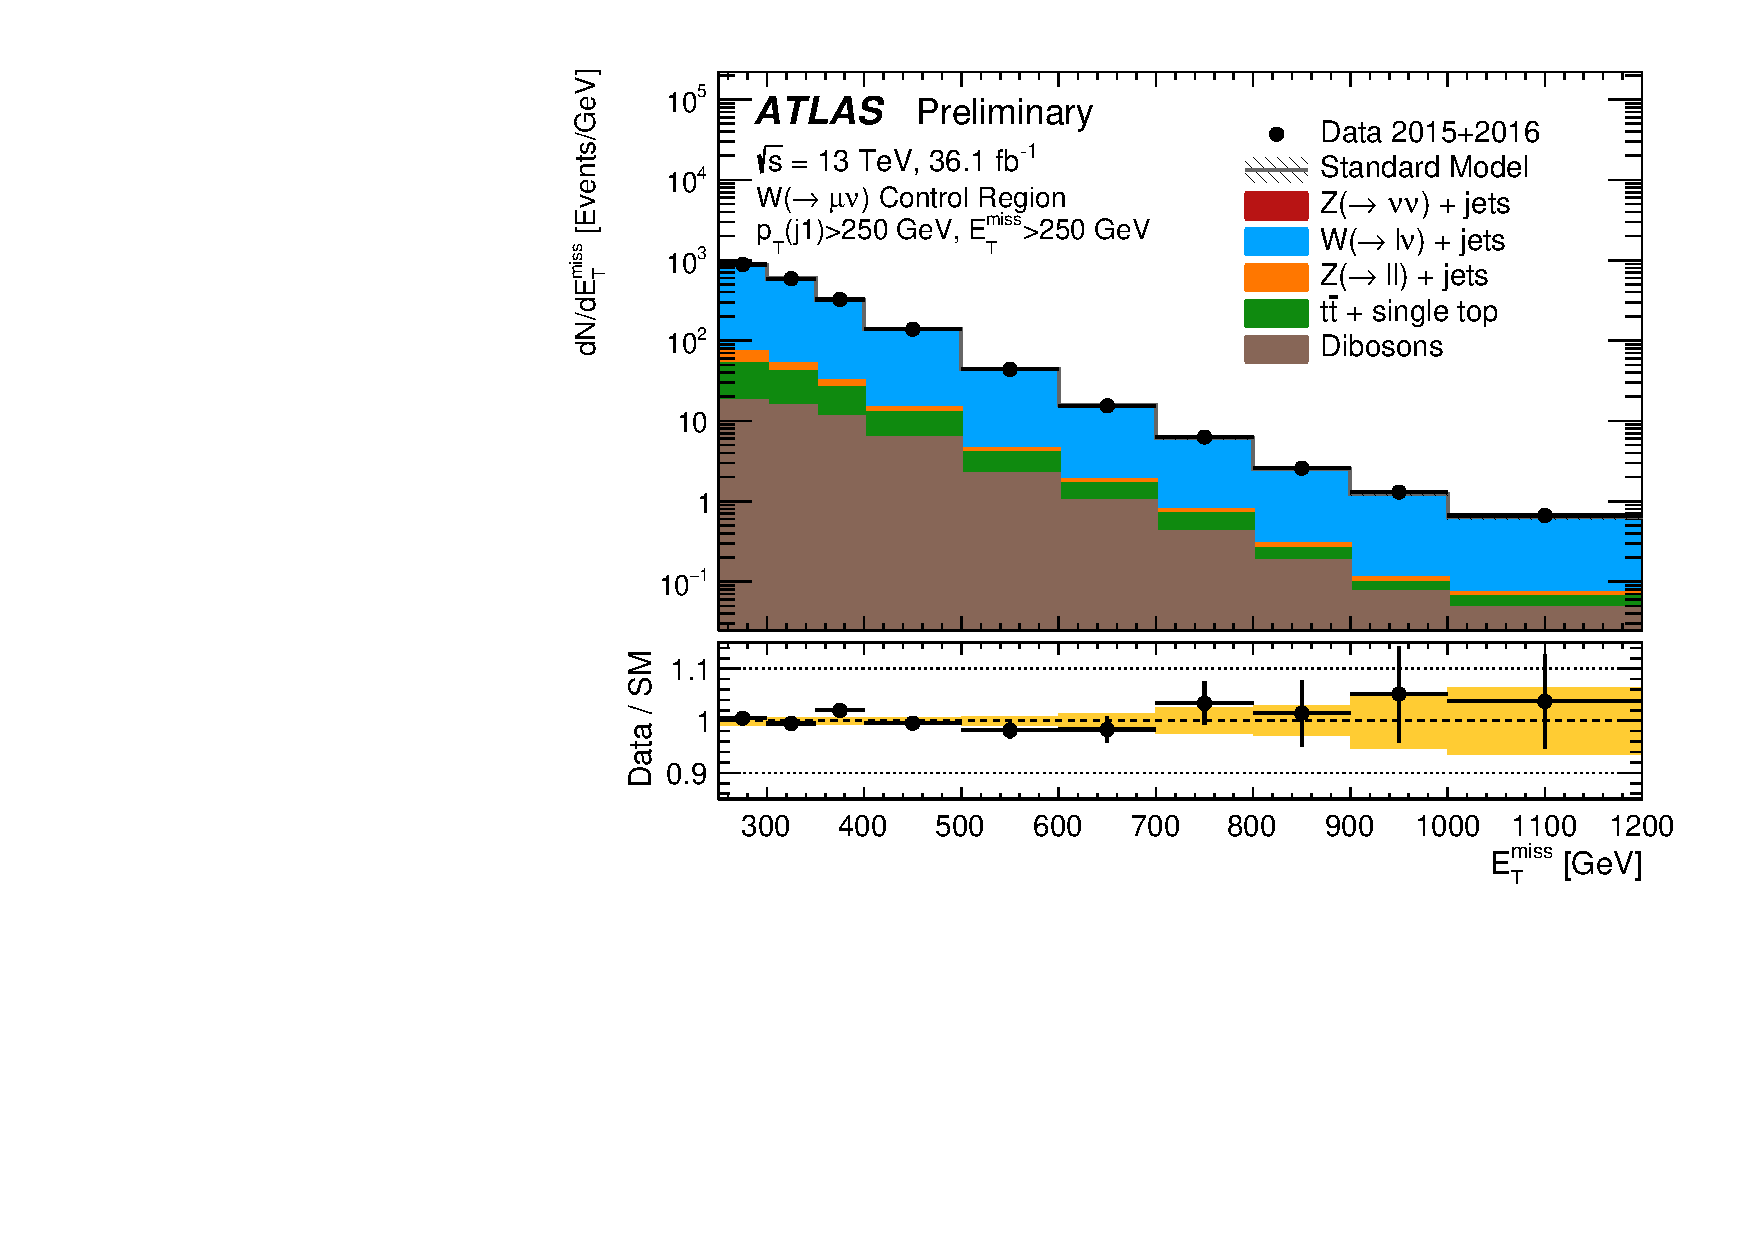
\includegraphics[width=\linewidth]{wmn_cr_met}
    \caption{$\met$ distribution.}
    \label{fig:wmn_cr_et_miss}
  \end{subfigure}
  \begin{subfigure}[t]{.48\linewidth}
    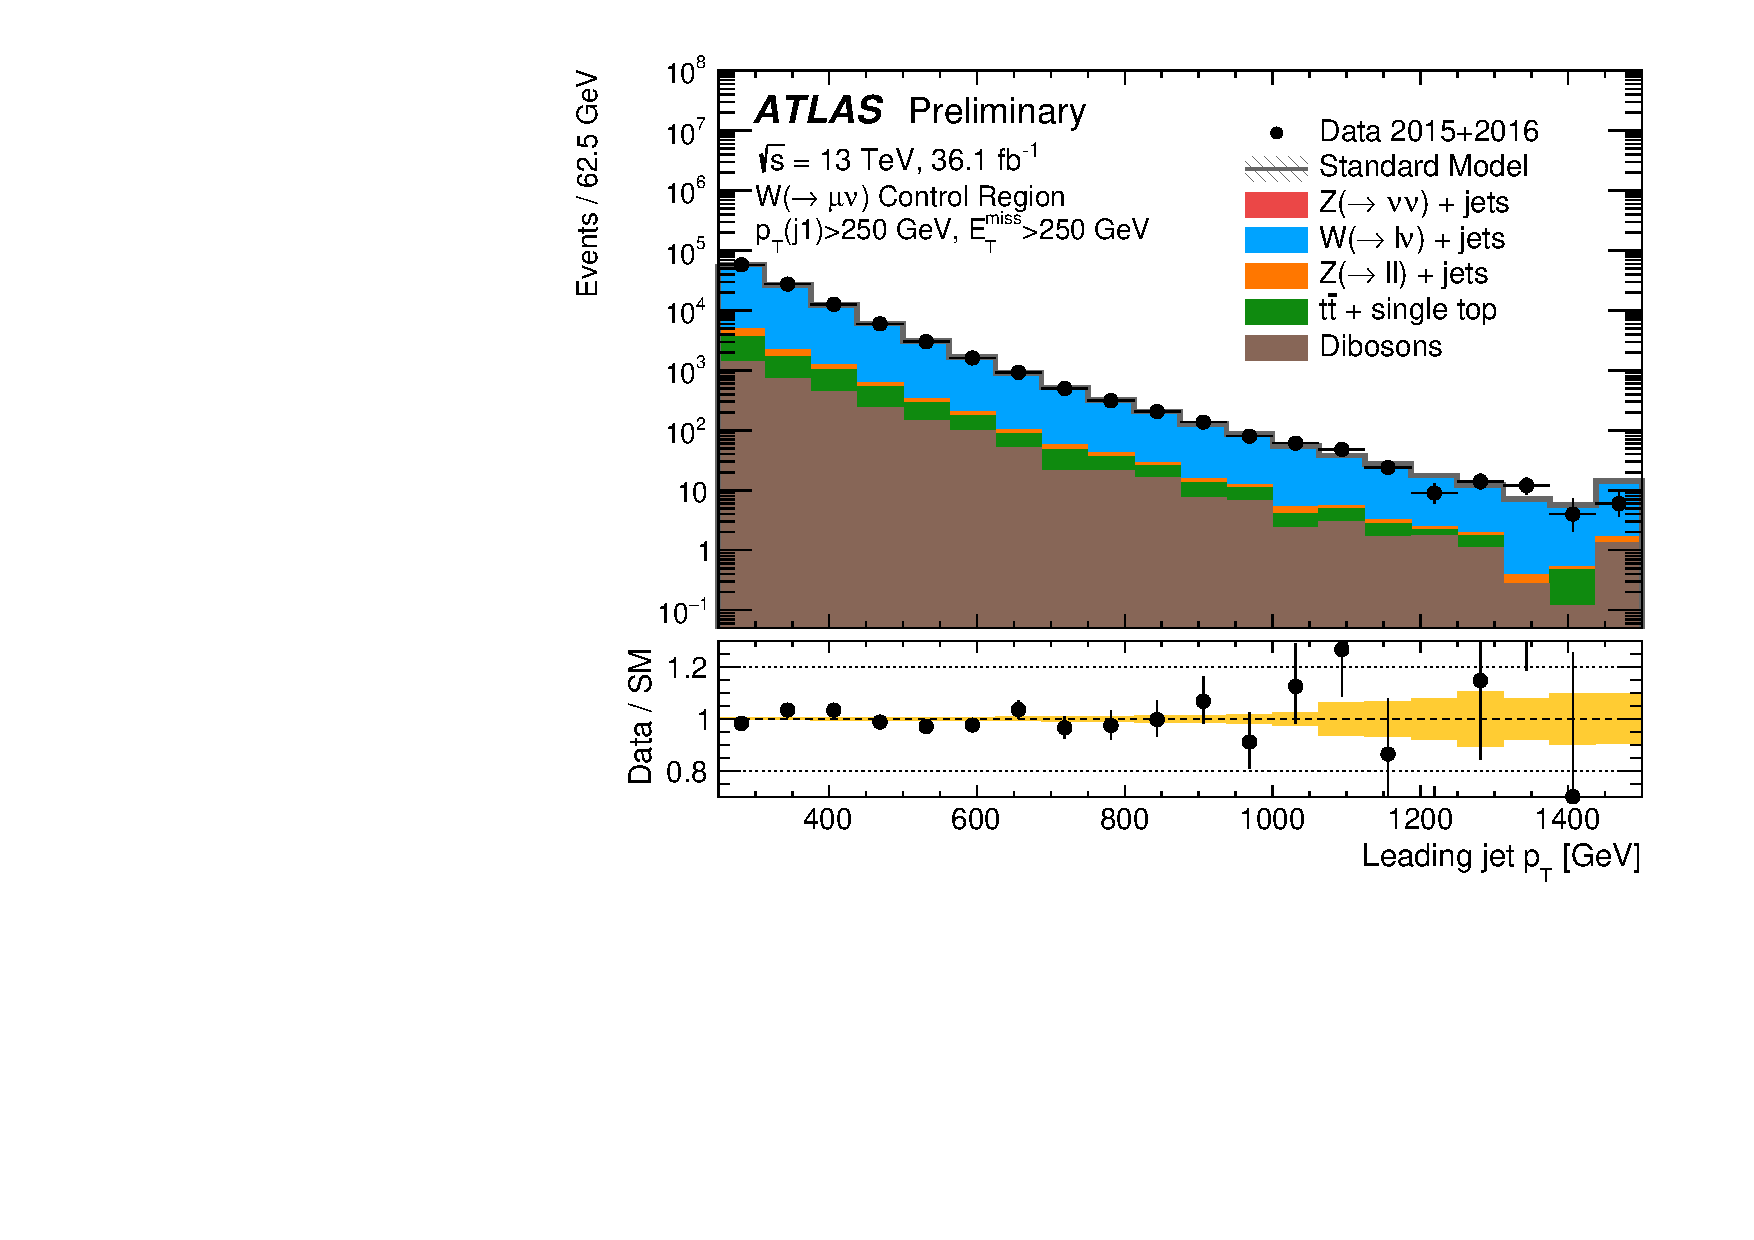
\includegraphics[width=\linewidth]{wmn_cr_jet1}
    \caption{Leading jet $\pt$ distribution.}
    \label{fig:wmn_cr_jet1}
  \end{subfigure}
  \caption{Observed and predicted $\met$ and leading jet $\pt$ after the
    background only fit in the $\crwmn$ control region for the $\met > 250$~GeV
    inclusive selection corresponding to IM1. The error bands in the ratio plot
    on the bottom of the figures include statistical and systematic
    uncertainties. The negligible contribution of \gls{ncb} and diboson
    backgrounds is not reported in the figure.}
  \label{fig:wmn_plots}
\end{figure}
%%% Local Variables:
%%% mode: latex
%%% TeX-master: "../search_for_DM_LED_with_ATLAS"
%%% End:
